\documentclass[a4paper,12pt]{article}
\usepackage[utf8]{inputenc}
\usepackage[english]{babel}
\usepackage{amsthm}
\usepackage{amsmath}
\usepackage{amssymb}
\usepackage{float}
\usepackage{enumitem}
\usepackage{url}
\usepackage[maxbibnames=99,backend=biber]{biblatex}
\usepackage{listings}
\usepackage{graphicx}
\graphicspath{ {imgs/} }
\usepackage{lscape}

\usepackage{courier}

\lstset{
basicstyle=\footnotesize\ttfamily,
breaklines=true
language=Python
}

\bibliography{rel}

%amsthm setup
\newtheoremstyle{newplanestyle}%                % Name
{10pt}%                                     % Space above
{0pt}%                                     % Space below
{\itshape}%                             % Body font
{}%                                     % Indent amount
{\bfseries}%                            % Theorem head font
{.}%                                    % Punctuation after theorem head
{ }%                                     % Space after theorem head, ' ', or \newline
{\thmname{#1}\thmnumber{ #2}\thmnote{ (#3)}} % Theorem head spec (can be left empty, meaning `normal')

\newtheoremstyle{newdefinitionstyle}%                % Name
{10pt}%                                     % Space above
{0pt}%                                     % Space below
{}%                             		  % Body font
{}%                                     % Indent amount
{\bfseries}%                            % Theorem head font
{.}%                                    % Punctuation after theorem head
{ }%                                    % Space after theorem head, ' ', or \newline
{\thmname{#1}\thmnumber{ #2}\thmnote{ (#3)}} % Theorem head spec (can be left empty, meaning `normal')

\newtheoremstyle{newprovestyle}%                 % Name
{10pt}%                                 % Space above
{0pt}%                                  % Space below
{}%                             		  % Body font
{}%                                     % Indent amount
{\itshape}%                            % Theorem head font
{.}%                                    % Punctuation after theorem head
{ }%                                    % Space after theorem head, ' ', or \newline
{} % Theorem head spec (can be left empty, meaning `normal')

\theoremstyle{newplanestyle}
\newtheorem{newtheo}{Theorem}[section]
\newtheorem{newprop}[newtheo]{Proposition}
\newtheorem{newlem}[newtheo]{Lem}
\newtheorem{newcor}[newtheo]{Corollary}

\theoremstyle{newdefinitionstyle}
\newtheorem{newdef}[newtheo]{Definition}
\newtheorem*{newdef*}{Definition}
\newtheorem{newex}[newtheo]{Example}

\theoremstyle{newprovestyle}
\newtheorem*{newprove}{Prove}

\addto{\captionsenglish}{\renewcommand{\abstractname}{Internship brief description}}

%opening
\title{%
  Asynchronous Approximate Distributed Computation for Machine Learning  \\
  First call report}
\author{Gianmarco Calbi}
\date{February 15, 2018}

\begin{document}
\maketitle

\section*{Context}
\subsection*{Machine learning training}
The most exploited method to train neural network is the Gradient Descent.

\subsection*{Gradient descent (GD)}
Iterative method to achieve a local optimum of a continuously differentiable function (\textit{convex/concave optimization always achieves \textbf{global} optimum}).

\begin{newdef*}[Empirical risk]
The \textit{empirical risk} $E_n$ is a function measuring the performance of the predicted model over the training set, is the one we'd like to minimize.
\[
E_n(\vec{w})=\frac{1}{n}\sum_{i=1}^{n}loss(f_{\vec{w}}(\vec{x}_i),y_i)
\]
\end{newdef*}
where:
\begin{itemize}
\item $n$ is the size of the training set;
\item the training set is defined as $\mathcal{X} = \{(\vec{x}_i, y_i) : i \in [n]\}$ where $\vec{x}_i$ is an input for the neural network and $y_i$ is the correct and desired output for such input;
\item $\vec{w}$ is the weight vector;
\item $loss(y_i, f_{\vec{w}}(\vec{x}_i))$ is the \textit{loss} function which measures the cost of predicting $f_{\vec{w}}(\vec{x}_i)$ (usually referred as $\hat{y_i}$) when the correct output should be $y_i$; obviously, $loss(y_i, \hat{y_i})=0 \Leftrightarrow \hat{y_i} = y_i$.
\end{itemize}

Several loss functions have been defined for different types of learning tasks, at the moment we are considering the \textit{squared loss function}:
\[
loss(y_i, \hat{y_i}) = \frac{1}{2}(y_i - \hat{y_i})^2
\]
so that $E_n$ is nothing but the \textit{mean squared error} of the trained function $f_{\vec{w}}(\vec{x})$ prediction over the training set.

GD is the most suitable method to achieve a $\vec{w}$ such that $f_{\vec{w}}$ can be retained a ``good'' approximation of the target function $y$. The \textit{goodness} of the approximation is directly related to $E_n$, usually when $E_n(\vec{w})$ get less than or equal to a user-defined small real number $\epsilon$ then $f_{\vec{w}}$ can be retained a good enough predictor.

GD method consists in a stepwise update of $\vec{w}$ starting from an initial $\vec{w}_0$ (either fixed or randomly picked):
\begin{equation*}
\vec{w}^{(t+1)} = \vec{w}^{(t)}-\alpha \nabla_{\vec{w}} E_n(\vec{w}^{(t)})
= \vec{w}^{(t)} - \frac{\alpha}{n} \sum_{i=1}^{n}(y_i - \hat{y}_i)(-\hat{y}_i)'
\end{equation*}
where $\alpha$ is the \textit{learning rate} (an higher learning rate value leads to fast convergence but less accurate solutions, while a smaller one do the opposite, it is always about finding a trade-off).

The computation is stopped either upon reaching a good enough solution (as explained before), or reaching a user-defined maximum number of iterations, or even stating divergence (this case may be avoided).

\subsection*{Stochastic gradient descent (SGD)}
When the size of the training set is such that the stepwise update of $\vec{w}$ requires an unaffordable computation effort, than one would rather rely on the \textit{stochastic gradient descent (SGD)}, that is a simplification of the classic method which outperforms GD w.r.t. single step speed and ensures (almost always under certain conditions) convergence, as well.

In SGD, the empirical risk $E_n$ computed on the whole training set $\mathcal{X}$, is replaced with $E(\vec{w})=loss(f_{\vec{w}}(\vec{x}_p),y_p)$ where $(\vec{x}_p, y_p)$ is a sample randomly picked from $\mathcal{X}$. Hence we aim to minimize the error just on a single sample rather than the error on the whole training set' samples. As stated before, under certain condition on the training set, approximating $E_n$ with $E$ will lead to converge as well.

The stepwise update of $w$ finally becomes
\[
\vec{w}^{(t+1)}=\vec{w}^{(t)}-\alpha \nabla_{\vec{w}} E(\vec{w}^{(t)})=\vec{w}^{(t)}-\alpha (y_p - \hat{y}_p)(-\hat{y}_p)'.
\]

\textit{Batch gradient descent (BGD)} behaves like GD but, instead of $E_n$, it computes $E_m$ by taking into account only a small subset of $\mathcal{X}$ of size $m$ instead of considering all the $n$ samples in the training set.

\subsection*{Training in a distributed environment}
Let the distributed system be composed of $k$ computational nodes, then the gradient descent is performed following the steps below:
\begin{enumerate}
\item the training set is split into $k$ disjoint subsets $\mathcal{X}_k$;
\item $\mathcal{X}_u$ is assigned to computational node $u$;
\item each node $u$, which owns a local weight vector $\vec{w}_u$, performs a single step update of it and obtains $\vec{w}^{(t)}_u$ ($w$ at $t$-th iteration);
\item then partial solutions from all nodes are averaged to a single $\vec{w}^{(t)}$;
\item each node updates his local model with $\vec{w}^{(t)}$;
\item repeat from 3 until a stop condition is met.
\end{enumerate}
In such kind of systems the weight update can be done either with GD or SGD, according to the size of the problem. Usually, the fact of working within a distributed system implicitly suggests that we're dealing with big datasets, therefore SGD is basically mandatory.


\subsection*{Bulk synchronous processing (BSP) gradient descent}
Nowadays distributed systems usually implement BSP model for SGD computation. In such model each node $u$ ending iteration $t$ (and producing $\vec{w}^{(t)}_u$) is forced to wait for all the others to finish, in order to average all outputs to a single weight vector $\vec{w}^{(t)}$; only after such shuffle phase (called barrier) a node can go on to the following step $t+1$.

\begin{newdef*}[Dependency graph]
Let $G=(V,E)$ be a digraph. $G$ is called a \textit{dependency graph} if its edges suggest a dependency relationship among vertices, e.g. $\forall e=(u,v) \in E$, $v$ ``depends on'' $u$. In our case, a dependency graph suggests that, for an iteration $t$, before to proceed to the following one, each node $v$ needs to average its own local weight vector with all its dependencies $u \in V : e=(u,v) \in E$ and $v \neq u$.
\end{newdef*}

\subsection*{Asynchronous gradient descent}
The dependencies among nodes within a BSP system can be rendered as a complete digraph $K_n = (V=[n],E=V \times V)$ composed of as many vertices as computational units in the system. The presence of a barrier after each stage (iteration) in BSP leads the overall computation dynamic to advance with time determined by slowest nodes. Indeed stragglers (nodes which experience a huge delay compared to the others) would heavely slow down the whole system. Removing barriers from BSP model should lead to straggler mitigation, e.g. an overall speed enhancement. The reasonable way to avoid barriers is to have few dependencies within the dep. graph.

\section*{Internship goal}
We're going to test different graphs' configurations to assess the advantages of an asynchronous model with respect to BSP. In particular we're interested in discovering a trade-off between amount of dependencies, convergence speed improvements and correctness of the solutions. 


\section*{Model overview}
We would like to emulate the behavior of a distributed system (that is a cluster of  machines running in parallel) within a single process (single-thread too, so far) to reproduce in details the distributed computation of SGD. Upon finding some interesting result we would also like to reproduce all tests on a real distributed environment.


\section*{Current results/outputs}

\subsection*{Model implementation progress}
At the moment the model can emulate a system with an arbitrary number of units computing either GD, SGD or BGD. The time taken by a node to perform a single step update of $w$ is determined by exploiting the exponential distribution.

\subsection*{Model setup}
Python application emulating a distributed system with 20 computational units.
\\
I have defined 3 different distributed model w.r.t dependency graph.

\subsubsection*{1) Complete graph (BSP)}
\begin{lstlisting}
n = 20
adjmat1 = GraphGenerator.generate_complete_graph(n)
cluster = Cluster(adjmat1)
\end{lstlisting}
\vspace{1em}

\subsubsection*{2) Cycle graph}
\begin{lstlisting}
n = 20
adjmat2 = GraphGenerator.generate_d_regular_graph_by_edges(
    n,
    ["i->i+1"]
)
cluster = Cluster(adjmat2)
\end{lstlisting}
Dependencies are set such that there is an edge from node $i$ to node $i+1$.
\vspace{2em}


\subsubsection*{3) A kind of expander graph}
\begin{lstlisting}
n = 20
adjmat3 = GraphGenerator.generate_d_regular_graph_by_edges(
    n,
    ["i->i+1", "i->i-1", "i->i+{}".format(int(n/2))]
)
cluster = Cluster(adjmat3)
\end{lstlisting}
Dependencies are set such that for node $i$ there are three edges $(i,i-1)$, $(i,i+1)$ and $(i,(i+10)\%20)$.
\vspace{2em}


\subsection*{Training set}
The training set is generated by exploiting the function below

\begin{lstlisting}
X, y = mltoolbox.sample_from_function(
    10000, 100, mltoolbox.LinearYHatFunction.f,
    domain_radius=10,
    domain_center=0,
    subdomains_radius=2,
    error_mean=0,
    error_std_dev=1,
    error_coeff=1
)
\end{lstlisting}

\begin{itemize}
\item \textit{10000}: samples in the training set;
\item \textit{100}: number of features;
\item \textit{mltoolbox.LinearYHatFunction.f}: target function used to compute the correct $y$ value for each $x \in \mathcal{X}$, in particular for this test is
\[f(x) = <X, \vec{w}>\]
\item the domain will be discussed in the next paragraph;
\item \textit{error}: noise added to each sample target function value:
\begin{lstlisting}
# pseudocode
# generate x matrix
noise = np.random.normal(error_mean, error_std_dev)
noise *= error_coeff
y[i] = f(x[i]) + noise
\end{lstlisting}
error coefficient equal to zero leads to a noiseless training set.
\end{itemize}

\paragraph*{Samples' domain.}
Since the target function is in the form $y=<X,\vec{w}>$, e.g.
\begin{equation*}
y_i = <X_i, \vec{w}> = \sum_{j=1}^{k}x_{ij}w_j,
\end{equation*}
then the error function assumes the form of a paraboloid.
To give evidence to our results, we would deal with functions on which SGD is supposed to be not trivial, so we are taking into account ill conditioned functions.

The actualization  of such idea consists in taking samples features values from different domain's ranges.

Let $k$ be the number of features, e.g. $k$ is the dimension of each sample $\vec{x} \in \mathcal{X}$, then for each $j \in \{1,...,k\}$, is randomly (from the uniform distribution) defined a compact $I_j \subset \mathcal{X}$ such that its radius is equal to \textit{subdomains radius}. The key point is to consider a subsamples radius of orders of magnitude smaller than the domain radius.

\textit{(Actually I have to do more study and research on this part from a theoretical point of view, so don't get stuck if it doesn't seems so clear.)} 

\subsection*{Training phase setup}

\begin{lstlisting}
cluster.setup(
    X, y, mltoolbox.LinearYHatFunction,
    max_iter=4000,
    method="stochastic", # "classic", "stochastic", or "batch"
    batch_size=20, #matters only for batch GD
    activation_func=None,
    loss=mltoolbox.SquaredLossFunction,
    epsilon = 0.01,
    alpha=0.0005,
    metrics="all",
    shuffle=True
)
\end{lstlisting}

\begin{itemize}
\item the maximum number of iterations is set to 4000 \textit{can be whatever one wants or can be even ``None'' or ``math.inf'' to never stop};
\item the method is set to stochastic but can be also batch or classic gradient descent;
\item batch size matters only is the method is set to batch;
\item activation function is set to ``None'', it means that the output is not normalized (the activation function is required for classification problems instead);
\item I am using the classical squared loss $\frac{1}{2}(y_i - \hat{y}_i)^2$ as loss function;
\item epsilon is the goodness threshold;
\item actually alpha is what I've always called ``learning rate'';
\item in metrics, one can specify the metrics the system should produce as output (mean squared error, mean average error, classification score, etc., or even ``all'' to compute all available metrics);
\item shuffle specify whether the cluster may shuffle the training set before doing anything else, it's important when one doesn't know whether and/or how the samples in the training set are ordered \textit{(usually it is worth to shuffle the training set whether not sure about its order)}.
\end{itemize}


I made everything from scratch (e.g. all the functions etc. used have been defined by me), so I have the complete control over every single instruction within the computation.

\section*{Sample tests}
\textit{Actually I experienced some issues in producing the metrics plots, therefore don't get mad to give an interpretation to the graphs below, just note that, as expected, the clique is the most accurate w.r.t. the number of iteration but is the worst if one considers the MSE over time; cycle and expander systems perform in a similar way but we are expecting that in future (and for sure more significant) tests this won't be so.}

\begin{landscape}
\centering
\subsection*{Global iterations over cluster clock}
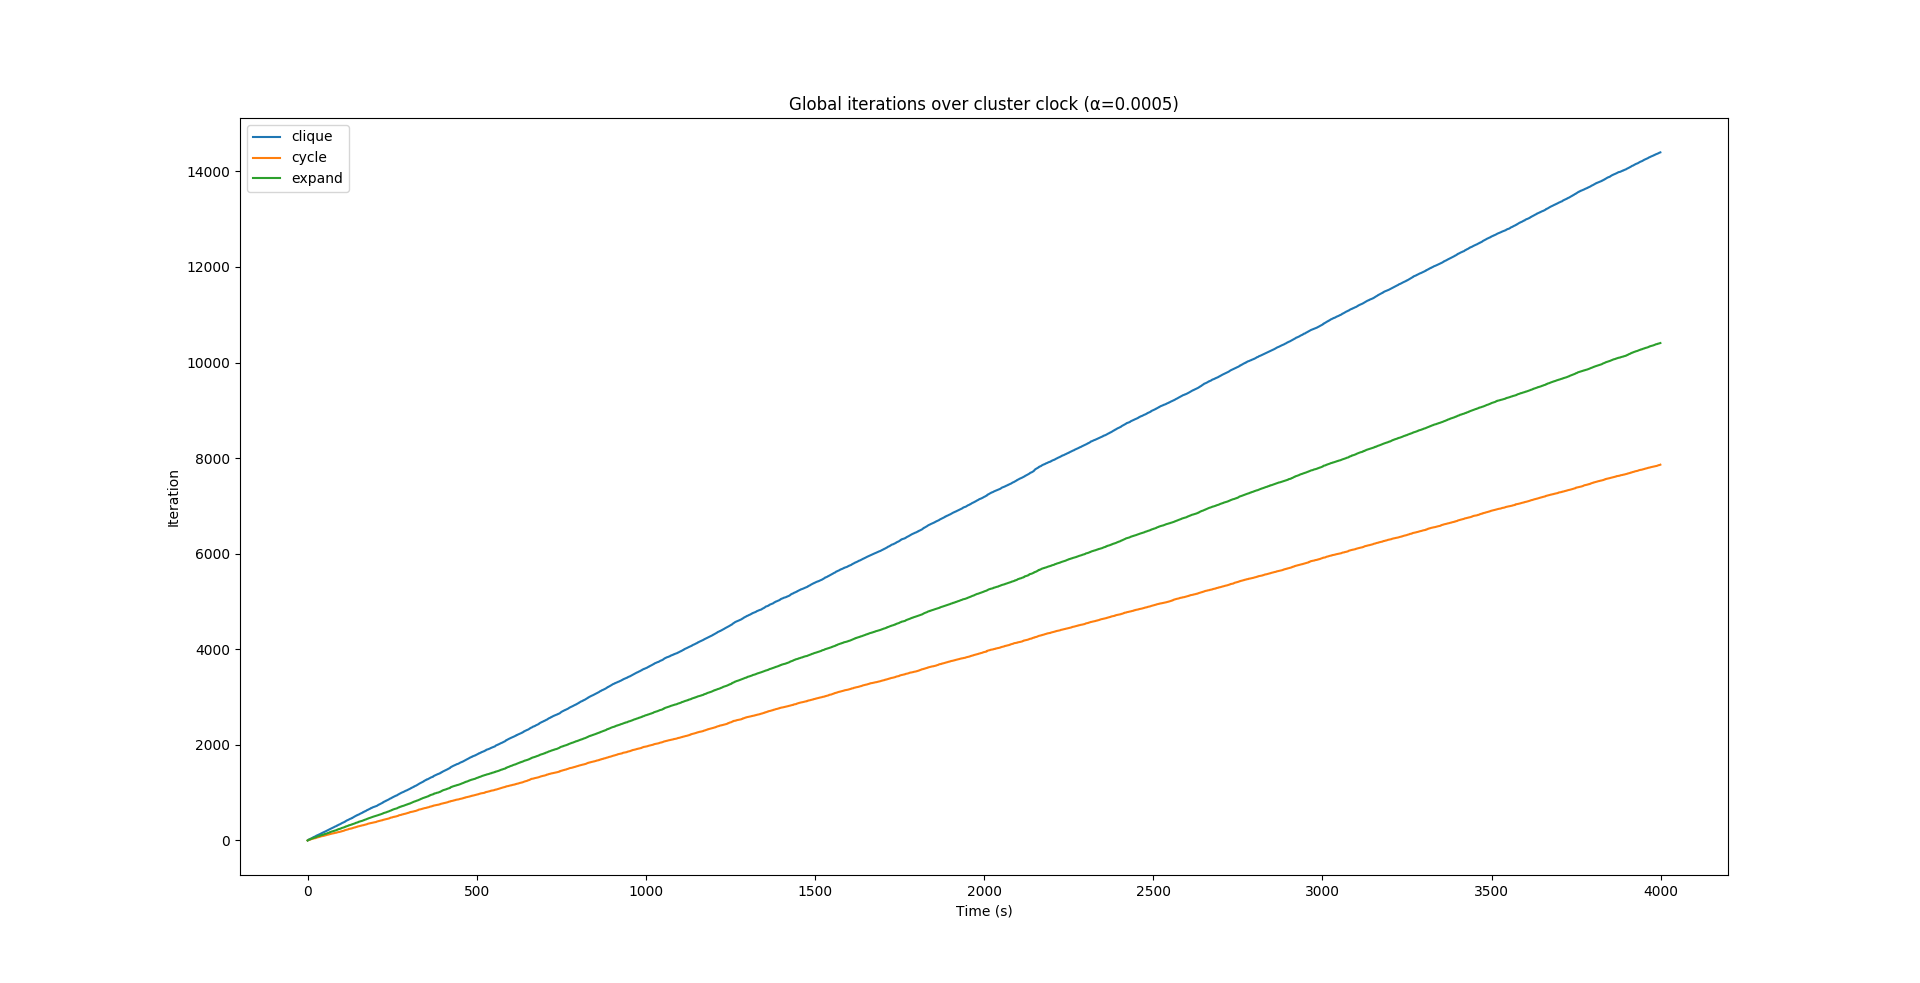
\includegraphics[scale=0.5]{iter_time_overview}

\centering
\subsection*{MSE over global iterations}
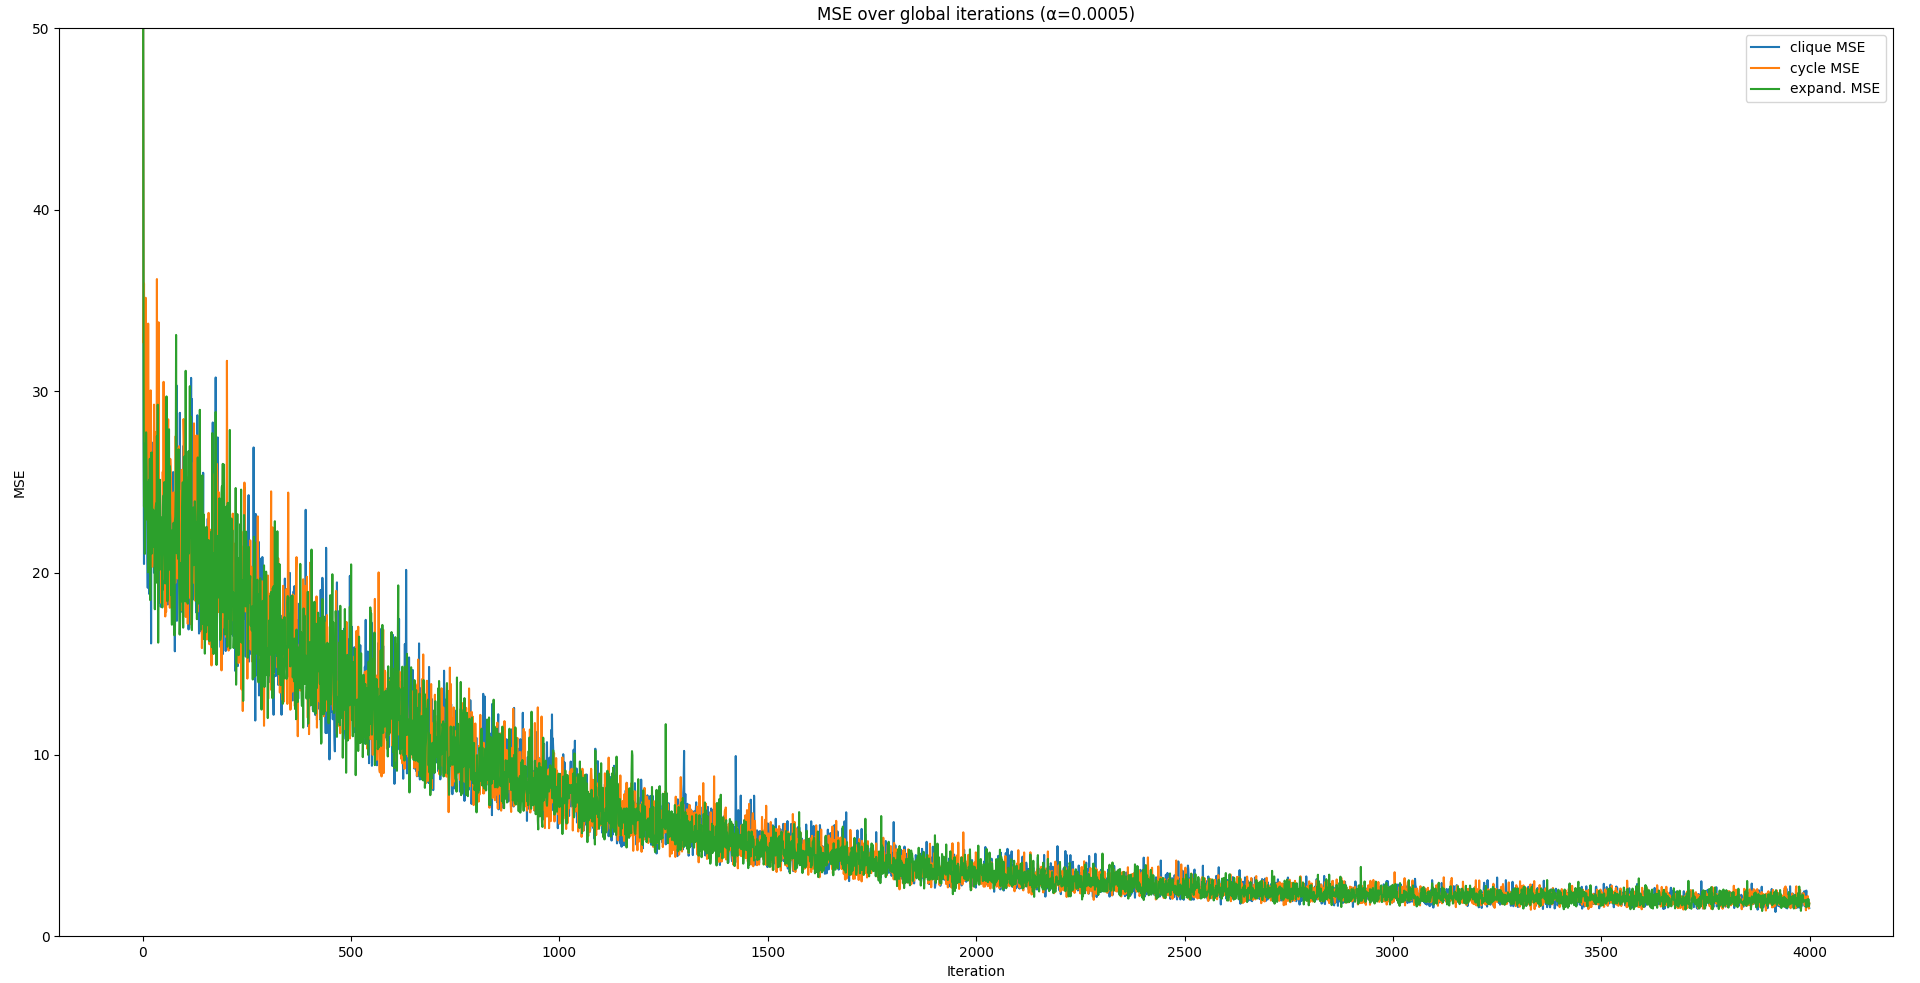
\includegraphics[scale=0.45]{mse_iter_overview}

\centering
\subsection*{MSE over cluster clock}
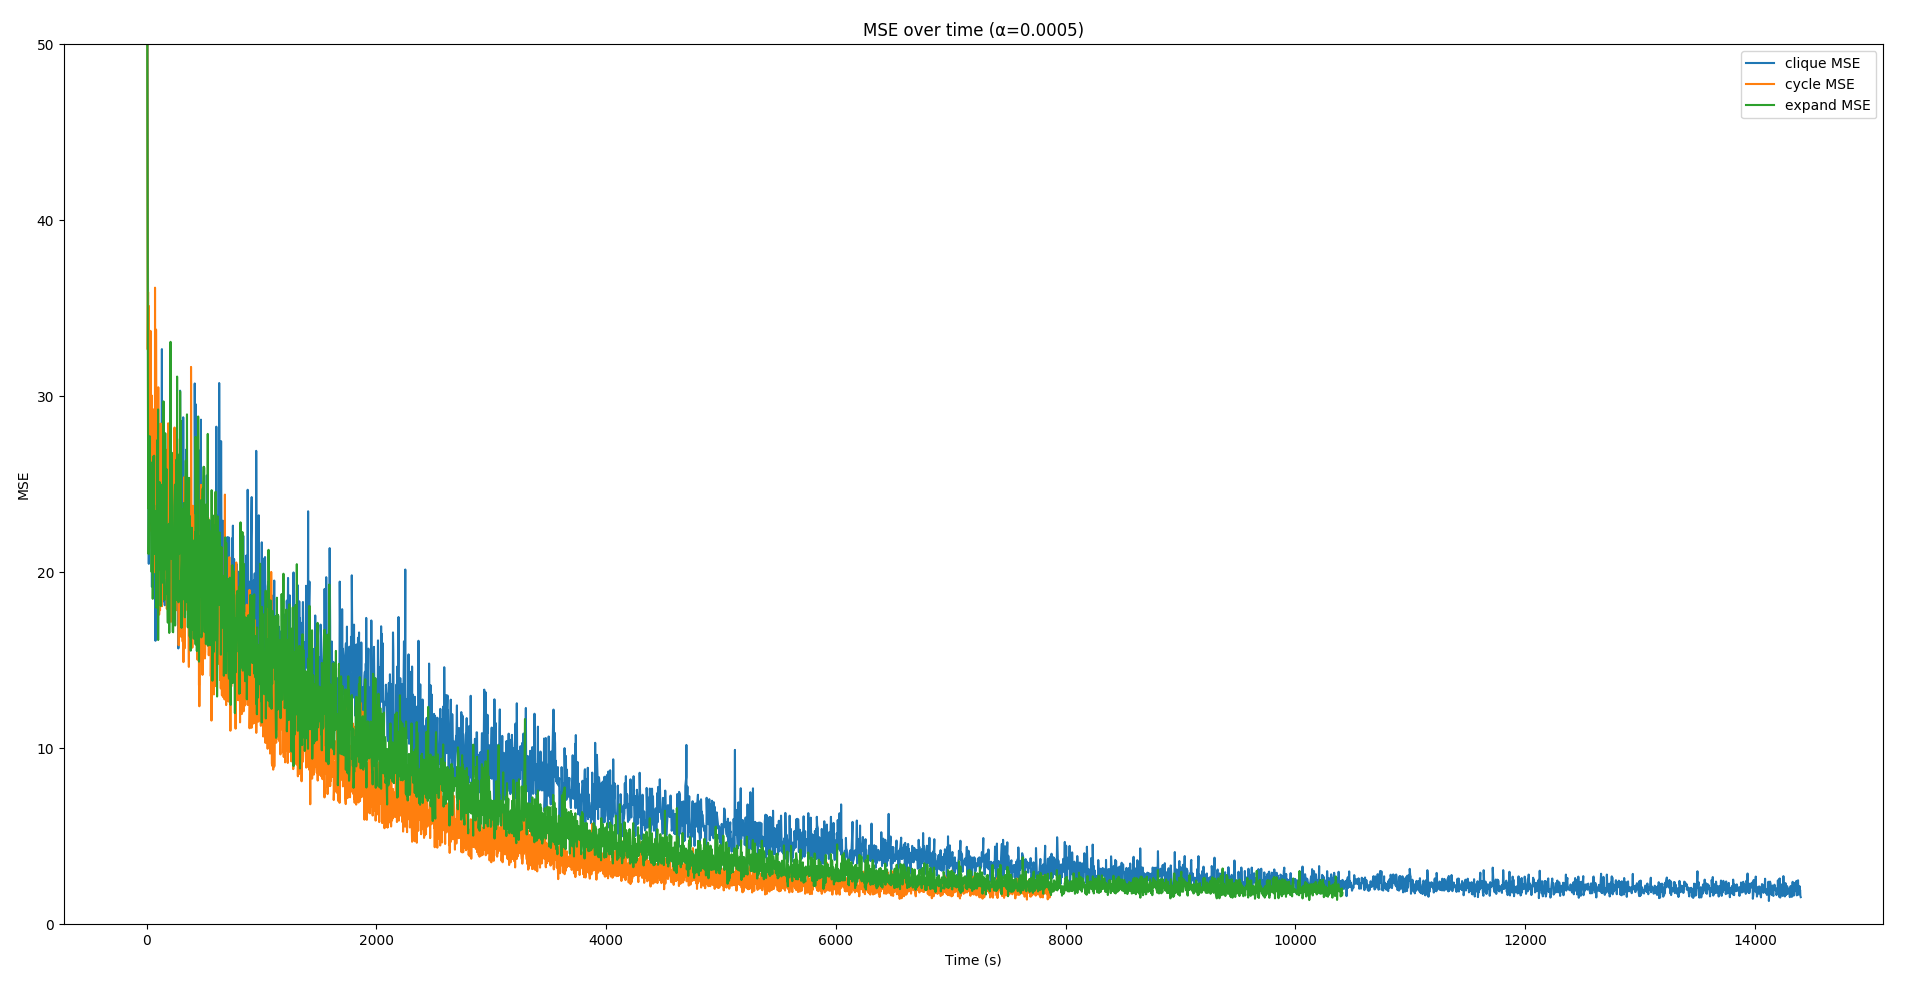
\includegraphics[scale=0.45]{mse_time_overview}
\end{landscape}

\end{document}
